\documentclass[a4paper]{article}

\usepackage[pages=all, color=black, position={current page.south}, placement=bottom, scale=1, opacity=1, vshift=5mm]{background}
\usepackage[margin=1in]{geometry} % full-width

% AMS Packages
\usepackage{amsmath}
\usepackage{amsthm}
\usepackage{amssymb}

% Unicode
\usepackage[utf8]{inputenc}
\usepackage{hyperref}
\hypersetup{
	unicode,
%	colorlinks,
%	breaklinks,
%	urlcolor=cyan, 
%	linkcolor=blue, 
	pdfauthor={ One, Author Two, Author Three},
	pdftitle={A simple article template},
	pdfsubject={A simple article template},
	pdfkeywords={article, template, simple},
	pdfproducer={LaTeX},
	pdfcreator={pdflatex}
}

% Vietnamese
%\usepackage{vntex}

% Natbib
\usepackage[sort&compress,numbers,square]{natbib}
\bibliographystyle{mplainnat}

% Theorem, Lemma, etc
\theoremstyle{plain}
\newtheorem{theorem}{Theorem}
\newtheorem{corollary}[theorem]{Corollary}
\newtheorem{lemma}[theorem]{Lemma}
\newtheorem{claim}{Claim}[theorem]
\newtheorem{axiom}[theorem]{Axiom}
\newtheorem{conjecture}[theorem]{Conjecture}
\newtheorem{fact}[theorem]{Fact}
\newtheorem{hypothesis}[theorem]{Hypothesis}
\newtheorem{assumption}[theorem]{Assumption}
\newtheorem{proposition}[theorem]{Proposition}
\newtheorem{criterion}[theorem]{Criterion}
\theoremstyle{definition}
\newtheorem{definition}[theorem]{Definition}
\newtheorem{example}[theorem]{Example}
\newtheorem{remark}[theorem]{Remark}
\newtheorem{problem}[theorem]{Problem}
\newtheorem{principle}[theorem]{Principle}

\usepackage{graphicx, color}
\graphicspath{{fig/}}

%\usepackage[linesnumbered,ruled,vlined,commentsnumbered]{algorithm2e} % use algorithm2e for typesetting algorithms
\usepackage{algorithm, algpseudocode} % use algorithm and algorithmicx for typesetting algorithms
\usepackage{mathrsfs} % for \mathscr command

\usepackage{lipsum}

% Author info
\title{Face Recognition}
\author{Vivek Sapkal$^1$ \and Kapil Yadav$^1$ \and Arsewad Bhagwan $^1$ \and Heramb Gavankar$^1$ \and Raj Patel$^1$ \and Suhani$^1$ \and Jateen$^1$}

\date{
	$^1$Indian Institute Technology, Jodhpur   \\ \texttt{\{b22ai066, b22ai024, b22ai010, b22ee028, b22ee053, b22cs051, b22cs026\}@iitj.ac.in}\\%
%	\today
}

\begin{document}
	\maketitle
	
	\begin{abstract}

 
This report presents the findings of a student project focused on exploring face recognition performance using the Labeled Faces in the Wild (LFW) People dataset. Face recognition technology holds significant relevance in various domains, including security, surveillance, and human-computer interaction. The LFW dataset, with its diverse collection of facial images sourced from the web, serves as a standard benchmark for evaluating face recognition algorithms.

The project begins by introducing the LFW dataset and discussing its characteristics, including image resolution, diversity of subjects, and variability in environmental conditions. The primary objective is to analyze the performance of different face recognition algorithms on this dataset and gain insights into their strengths and limitations.

Various methodologies, including traditional machine learning methods are explored and implemented for comparison. The project investigates the impact of factors such as pose variation, lighting conditions, and facial expressions on recognition accuracy through systematic experiments and evaluations.

Moreover, the report discusses the challenges encountered during the project, such as data preprocessing, model selection, and parameter tuning, along with the strategies adopted to address them. Additionally, the importance of experimental rigor, including cross-validation techniques and performance metrics, is emphasized to ensure the validity and reliability of the results.

Through this project, students aim to enhance their understanding of fundamental concepts in face recognition while gaining practical experience in implementing and evaluating traditional machine learning algorithms. The insights and lessons learned from this endeavor contribute to their academic growth and readiness for future research or professional pursuits in the field of computer vision and machine learning.	
		\vspace{10cm}	
		\noindent\textbf{Keywords:} Face Recognition, LFW dataset, Machine Learning
	\end{abstract}

	\tableofcontents
	
	\section{Introduction}
	\label{sec:intro}

 
In this project, we focus on the task of face recognition using the Labeled Faces in the Wild (LFW) People dataset, a widely used benchmark in the field.

The LFW dataset consists of thousands of facial images collected from the web, featuring a diverse set of individuals in various poses, lighting conditions, and facial expressions. Our goal is to evaluate and improve the performance of face recognition algorithms on this dataset, considering the challenges posed by real-world scenarios.

Firstly, we observed notable improvements in model performance by employing oversampling and augmentation techniques to address data imbalance issues present in the LFW dataset.

Additionally, we explored the effectiveness of feature extraction methods such as Histogram of Oriented Gradients (HOG), Local Binary Patterns (LBP), and features extracted from pre-trained ResNet models. These features proved to enhance recognition accuracy when integrated into our models.

Furthermore, dimensionality reduction techniques, particularly Principal Component Analysis (PCA), were applied to reduce the computational complexity and improve the efficiency of our models.

Moreover, we experimented with ensemble learning techniques, combining predictions from multiple models to achieve superior performance compared to individual classifiers. The ensemble approach demonstrated robustness and resilience to variations in the dataset, leading to improved overall accuracy.

In this report, we present a detailed analysis of our methodologies, experimental findings, and insights gained from the project. The structure of the report is as follows: Section \ref{sec:app} discusses the various approaches we explored in our quest to improve face recognition performance. Section \ref{sec:exp} presents the experimental setup, dataset details, and comparative results. Finally, Section \ref{sec:summ} summarizes the key findings and contributions of our project.
	

 \newpage
	\subsection{Figures}
    \begin{figure}[!htb]
    \centering
    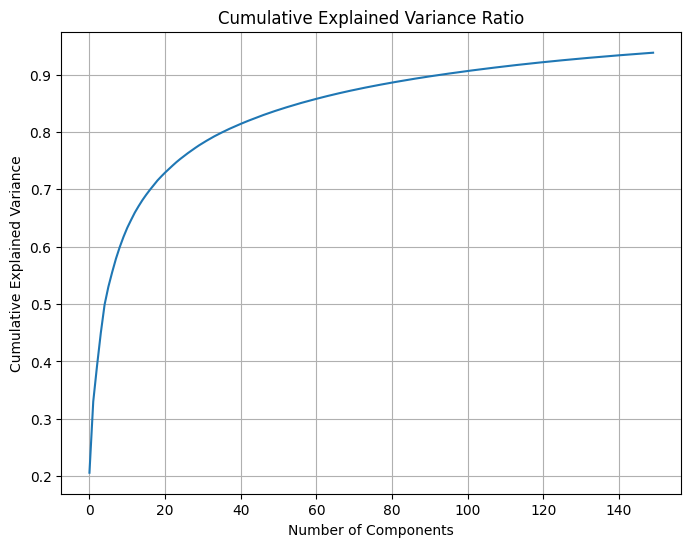
\includegraphics[width=0.8\textwidth]
    {figs/explained variance ratio.png}
    \caption{Cumulative explained variance by Principal components}
    \label{fig:img1}
\end{figure}

    \begin{figure}[!htb]
    \centering
    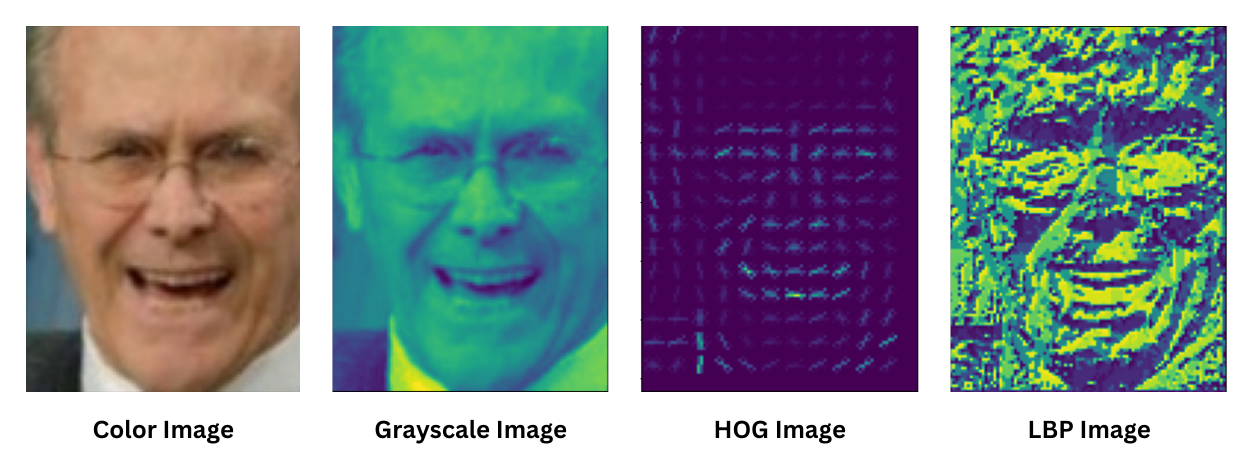
\includegraphics[width=0.8\textwidth]
    {figs/Image transforms.png}
    \caption{Images with various feature representations}
    \label{fig:img2}
\end{figure}

    \begin{figure}[!htb]
    \centering
    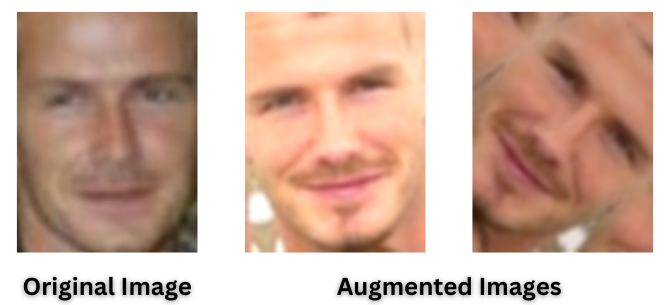
\includegraphics[width=0.6\textwidth]
    {figs/Augmented Images comparsion.png}
    \caption{Augmented Images}
    \label{fig:img3}
\end{figure}

	\begin{figure}[!htb]
        \centering
        \includegraphics[width=0.8\textwidth]{figs/accuracies_comparison_plots.png}
        \caption{ Model trained on 62 classes.}
        \label{fig:img4}
    \end{figure}

    \begin{figure}[!htb]
    \centering
    \includegraphics[width=0.8\textwidth]{figs/accuraciec_comparison_plots_100_min.png}
    \caption{Model trained on 5 classes.}
    \label{fig:img5}
\end{figure}

    \begin{figure}[!htb]
    \centering
    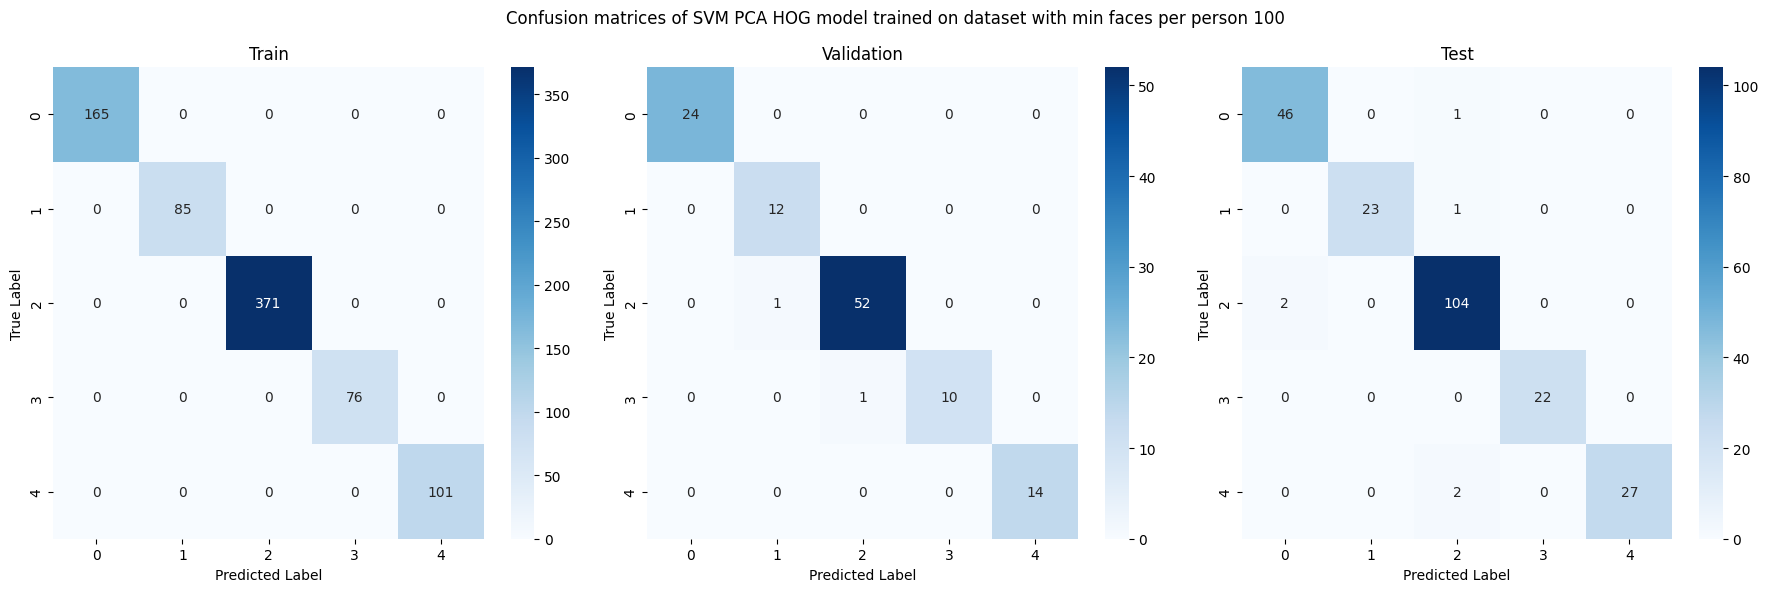
\includegraphics[width=0.8\textwidth]
    {figs/confusion_matrices_svm_pca_hog_min_100.png}
    \caption{Confusion matrices of SVM PCA HOG model trained on dataset with 5 classes}
    \label{fig:img5}
\end{figure}

\clearpage
	
	\section{Approaches Tried}
	\label{sec:app}

        Throughout our experimentation, we explored a diverse range of methodologies aimed at enhancing face recognition performance on the challenging LFW People dataset. We started out with keeping minimum 20 images per person from the dataset. This gave us 3023 images of 62 people. We observed class imbalance in the dataset. We then used the dataset with at minimum 100 images per person. This gave us 1140 images of 5 people. In Both the cases the dataset has class imbalance as images of some people are in vast majority.
        
        Below, we provide detailed descriptions of the approaches we pursued:

\subsection{SMOTE Oversampling}
   \begin{itemize}
       \item Addressing the class imbalance inherent in the dataset, we applied the Synthetic Minority Over-sampling Technique (SMOTE) to generate synthetic samples for minority classes.
       \item SMOTE oversampling generated synthetic images of minority classes such that the total number of images in each class became equal to maximum number of images of any class in the train set. Thus the total number of images became 371 per person.
   \end{itemize}

\subsection{Data Augmentation}
   \begin{itemize}
       \item  To enrich training diversity, we employed extensive augmentation techniques. Our augmentation included diverse transformations such as rotation, flipping and brightness and contrast changes with certain probabilities.
       \item  We aimed for 200 images per class to ensure dataset uniformity. Augmented classes with fewer than 200 images to mitigate imbalance. Randomly selected and transformed images to generate new samples. 
       \item For classes with more than 200 images, 200 images were randomly selected.
   \end{itemize}
   
\subsection{PCA Transformation}
   \begin{itemize}
       \item Subsequently, to reduce the dimensionality of the feature space and mitigate the curse of dimensionality, we employed Principal Component Analysis (PCA) for effective dimensionality reduction. 
       \item The flattened RGB images conatined 35250 pixel values. We applied PCA with 100 principal components to reduce dimensionality while preserving most of the variance in the dataset.
   \end{itemize}
   
\subsection{KNN and SVM Models with PCA Transformation}
   \begin{itemize}
       \item Utilizing the PCA-transformed data, we trained k-Nearest Neighbors (KNN) and Support Vector Machine (SVM) classifiers.
       \item Employing an exhaustive grid search approach, we identified the optimal hyperparameters for each model. The best configurations included selecting 1 neighbor for KNN and utilizing an RBF kernel with a regularization parameter (C) value of 10 for SVM.
   \end{itemize}

\subsection{MLP on PCA-Transformed Data}
   \begin{itemize}
       \item Leveraging the expressive power of neural networks, we applied a Multi-Layer Perceptron (MLP) architecture to the PCA-transformed data.
       \item The MLP model comprised two hidden layers, allowing for the learning of complex patterns in the reduced-dimensional feature space. This approach yielded significant performance improvements over traditional classifiers such as KNN and SVM.
   \end{itemize}

\subsection{HOG Feature Extraction and MLP}
   \begin{itemize}
       \item Employing the Histogram of Oriented Gradients (HOG) technique, we extracted informative features capturing local image gradients and textures. We set the hyperparameters of the model to have 9 orientation bins, (8, 8) pixels per cell and (2, 2) cells per block.
       \item PCA transformation was applied to the extracted HOG features with 100 principal components.
       \item SVM model was applied to the PCA transformed HOG features observing notable enhancements in performance.
       \item We then fed the raw HOG features and PCA-transformed HOG features into MLP neural networks.
   \end{itemize}

\subsection{LBP Feature Extraction and Classification}
   \begin{itemize}
       \item Extracting Local Binary Patterns (LBP) features from grayscale images, we aimed to capture texture information crucial for face recognition.
       \item We applied PCA with 100 principal components to reduce dimensionality while preserving most of the variance in the dataset.
       \item Following PCA transformation of the LBP features, we evaluated the performance of SVM, and MLP classifiers.
   \end{itemize}

\subsection{ResNet50 Feature Extraction and Classification}
   \begin{itemize}
       \item Leveraging the power of deep learning, we extracted features using the ResNet50 architecture, a state-of-the-art convolutional neural network pre-trained on large-scale image datasets.
       \item The ResNet50 model was loaded and its last layer was removed. Then the model was used to extract features from our dataset. 
       \item KNN and SVM were trained on the PCA transformed resnet extracted features and MLP was trained on both raw resnet extracted features and PCA transformed resnet extracted features.
   \end{itemize}

\subsection{Ensemble Methods}
   \begin{itemize}
       \item In pursuit of enhanced robustness and generalization, we constructed ensembles by aggregating predictions from individual models through majority voting.
       \item Furthermore, we explored an ensemble approach wherein the predictions of all models were treated as additional features, and a Random Forest classifier was employed to learn the complex relationships between these features and the target labels.
   \end{itemize}

These comprehensive approaches encompassed various techniques spanning oversampling, dimensionality reduction, feature extraction, and ensemble learning, aimed at pushing the boundaries of face recognition performance on the challenging LFW People dataset.
	\newpage
 
	\section{Experiments and Results}
	\label{sec:exp}
	Write about dataset, experimental setting, compare results
	
\subsection{Dataset Description}


Labeled Faces in the Wild (LFW) is a database of face photographs designed for studying the problem of unconstrained face recognition. This database was created and maintained by researchers at the University of Massachusetts, Amherst. 13,233 images of 5,749 people were detected and centered by the Viola Jones face detector and collected from the web. 1,680 of the people pictured have two or more distinct photos in the dataset. The dataset presents several challenges, including variations in pose, illumination, facial expression, and image resolution.

\subsection{Experimental Settings}

We used the dataset keeping varying criteria for minimum number of images per person. We started out minimum 20 images per person. Here we got 3023 images of 62 peoples. We also trained models on dataset with minimum 100 images per person. Here we got 1140 images of 5 people. 

\subsubsection{Preprocessing}

The dataset was used with both grayscale and RGB images. The grayscale iamges were used for extarcting HOG and LBP features. Dataset with resized images was also used to train some models. The dataset was split into train, validation and test sets in the ratio 70:10:20 respectively. Oversampling and Data augmentation was done only on train sets. Traditional ML methods such as KNN, SVM, MLP, PCA along with HOG, LBP and Resnet feature extraction was performed. we used various Python libraries including but not limited to: numpy, pytorch, matplotlib, Albumtetations, sklearn, etc.Models were evaluated for Accuracy on train and tests.

\subsection{Results}

The experimental results demonstrate the effectiveness of the proposed methodologies in enhancing face recognition performance on the LFW dataset. Comprehensive analyses of model performance under various experimental settings are presented, highlighting the impact of oversampling, augmentation, feature extraction, dimensionality reduction, and ensemble learning techniques.

Further details regarding the experimental setup, evaluation metrics, and comparative results are provided in subsequent subsections.

\subsubsection{Accuracy Tables}

\begin{table}[htbp]
    \centering
    \begin{tabular}{|c|c|c|c|}
    \hline
    \textbf{Features} & \textbf{Baseline} & \textbf{Oversampling} & \textbf{Augmentation}\\
    \textbf{} & \textbf{Train/Test Acc} & \textbf{Train/Test Acc} & \textbf{Train/Test Acc }\\
    \hline
    KNN PCA & 100 / 31.2 & 100 / 31.23 & 100 / 28.59 \\
    \hline
    SVM PCA & 99.85 / 55.5 & 100 / 53.05 & 99.88 / 53.71 \\
    \hline
    MLP PCA & 95.31 / 59.66 & 100 / 61.15 & 97.48 / 59.50 \\
    \hline
    SVM PCA HOG  & 100 / 69.58 & 100 / 69.58 & 100 / 73.22 \\
    \hline
    MLP HOG & 97.2 / 67.9 & 100 / 70.74 & 97.34 / 71.73 \\
    \hline
    MLP PCA HOG & 82.5 / 63.6 & 98.92 / 66.28 & 75.04 / 61.65 \\
    \hline
    SVM PCA LBP & 100 / 53.7 & 100 / 48.42 & 100 / 59 \\
    \hline
    MLP PCA LBP & 95.27 / 34.7 & 79.45 / 42.64 & 89.36 / 43.47 \\
    \hline
    SVM PCA Resnet & 67.89 / 33.55 & 100 / 33.05 & 100 / 29.58 \\
    \hline
    KNN PCA Resnet & 40.75 / 19.83 & 100 / 15.70 & 100 / 13.55 \\
    \hline
    MLP Resnet & 58.62 / 35.70  & 97.37 / 36.52 & 64.45 / 32.89  \\
    \hline
    MLP PCA Resnet & 69.69 / 37.00  & 100 / 37.70 & 94.01 / 34.21 \\
    \hline
    Ensemble (RF) & 100 / 51.07 & 100 / 64.29 & 100 / 64.79 \\
    \hline
    Ensemble (Voting) & 99.99 / 70.57 & 100 / 71.23 & 100 / 77.85 \\
    \hline
    \end{tabular}
    \caption{Accuracies on Datasets with min 20 faces per person with 62 persons}
    \label{tab:accuracy1}
\end{table}

\begin{table}[htbp]
    \centering
    \begin{tabular}{|c|c|c|c|}
    \hline
    \textbf{Features} & \textbf{Baseline} & \textbf{Oversampling} & \textbf{Augmentation}\\
    \textbf{} & \textbf{Train/Test Acc} & \textbf{Train/Test Acc} & \textbf{Train/Test Acc }\\
    \hline
    KNN PCA & 73.30 / 60.96 & 100 / 57.01 & 100 / 56.14 \\
    \hline
    SVM PCA & 100 / 87.19 & 100 / 85.96 & 100 / 86.40 \\
    \hline
    MLP PCA & 91.35 / 78.94 & 98.92 / 84.84 & 98.2 / 85.52 \\
    \hline
    SVM PCA HOG  & 100 / 97.36 & 100 / 93.85 & 100 / 94.73 \\
    \hline
    MLP HOG & 98.62 / 90.78 & 99.89 / 92.98 & 99 / 93.42 \\
    \hline
    MLP PCA HOG & 98.74 / 90.35 & 98.43 / 93.85 & 93.8 / 90.78 \\
    \hline
    SVM PCA LBP & 100 / 78.50 & 99.99 / 69.29 & 100 / 82.45 \\
    \hline
    MLP PCA LBP & 100 / 76.75 & 100 / 72.36 & 100 / 67.10 \\
    \hline
    SVM PCA Resnet & 84.58 / 71.49 & 100 / 70.61 & 100 / 66.66 \\
    \hline
    KNN PCA Resnet & 68.67 / 53.94 & 100 / 46.05 & 100 / 43.42 \\
    \hline
    MLP Resnet & 72.56 / 65.78 & 90.24 / 72.36  & 78.8 / 67.10  \\
    \hline
    MLP PCA Resnet & 96.37 / 91.92 & 99.57 / 71.05 & 96.2 / 64.91 \\
    \hline
    Ensemble (RF) & 100 / 92.98 & 100 / 89.47 & 100 / 90.78 \\
    \hline
    Ensemble (Voting) & 100 / 92.98 & 100 / 91.22 & 100 / 93.85 \\
    \hline
    \end{tabular}
    \caption{Accuracies on Datasets with min 100 faces per person with 5 different persons}
    \label{tab:accuracy1}
\end{table}
	
\subsubsection{Interpretation of Results}

\begin{itemize}

    \item Simple representations like PCA may not capture intricate facial details, resulting in lower accuracy compared to more complex representations like HOG.
    
    \item Model performance varies notably across different feature representations and augmentation techniques, with SVM PCA HOG and Ensemble (Voting) consistently achieving high test accuracies.
    
    \item Data augmentation introduces variability, aiding in better model generalization, as observed in MLP PCA HOG's performance improvement.
    
    \item Ensemble methods, such as Random Forest and Voting, are effective in mitigating individual model biases and errors, leading to more robust predictions that consistently perform well across various scenarios by leveraging diverse model predictions.
    
    \item Significant improvements in accuracies were observed after oversampling and data augmentation for models trained with the LFW dataset with a minimum of 20 images per person (62 classes and very high class imbalance).
    
    \item For models trained with the LFW dataset with a minimum of 100 images per person (5 classes and low class imbalance), marginal improvements or even decreases in accuracies were observed after oversampling and augmentation.
    
\end{itemize}

	\section{Summary}
	\label{sec:summ}

Throughout this project, our aim was to enhance face recognition performance on the challenging LFW People dataset. We addressed class imbalance using SMOTE and augmented the dataset for robustness. Various feature extraction methods like HOG, LBP, and ResNet50 were explored, with PCA used for dimensionality reduction. Traditional ML models (KNN, SVM, MLP) were trained on both raw pixels and extracted features, with hyperparameter optimization conducted via grid search.

Ensemble learning methods such as majority voting and Random Forest were employed to combine model predictions for improved accuracy and robustness. The experimental results demonstrated significant improvements in accuracy compared to baseline models, highlighting the impact of oversampling, augmentation, feature extraction, dimensionality reduction, and ensemble learning techniques.

By leveraging diverse approaches and traditional ML methodologies, the project aimed to advance face recognition on challenging datasets like LFW People, with implications for real-world applications requiring accurate facial recognition.
	
	\bibliography{refs}
\cite{AnalyticaVidhya}
\cite{Medium_aricle}
\cite{Neural_network}
\cite{CNNResnet}

	\appendix
	
	\section{Contribution of each member}
	\label{sec:contribution}
	\begin{enumerate}
	\item Vivek Sapkal: Implemented HOG, LBP feature extractions and SVM on various feature representations and made the report.
	\item Kapil Yadav: Implemented Resnet-50 feature extraction, Data Augmentation and made the project page, Demo code and report.
 	\item Bhagwan Arsewad: Implemented MLP on various feature representations and prepared video recording.
	\item Heramb Gavankar: Implemented PCA on various feature representations and prepared video recording. 
	\item Raj Patel: Implemented KNN on various feature representations.
	\item Suhani: Implemented plotting of various plots for analysis and contributed in preprocessing.
	\item Jateen: Implemented Oversampling and wrote readme file for github.
	\end{enumerate}
    	
	
\end{document}
